\documentclass[tikz,border=5pt]{standalone}
\usepackage{amsmath}
\usetikzlibrary{arrows.meta,calc}
\tikzset{arr/.style={-{Stealth[length=2.2mm]},thick},ray/.style={arr,orange!80!black},hidden/.style={gray!55,densely dashed}}
\begin{document}
% Orthographic projection columns: x=(cos30,-sin30 sin20),
% y=(-sin30,-cos30 sin20), z=(0,cos20). Viewer=(.46985,.81380,.34202).
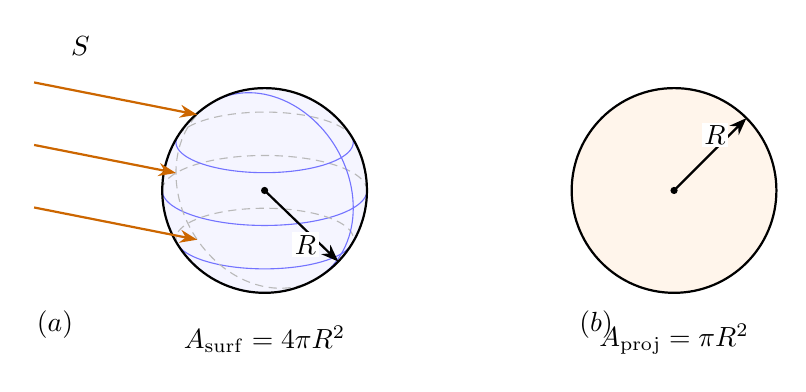
\begin{tikzpicture}[font=\normalsize,scale=1.3]
  \coordinate (C) at (0,0);
  \fill[blue!4] (C) circle (1);
  \foreach \zz/\aa in {0/90,.5/102.1,-.5/77.9}{
    \pgfmathsetmacro{\rr}{sqrt(1-\zz*\zz)}
    \draw[hidden] plot[domain={60+\aa}:{420-\aa},samples=61]
      ({\rr*(.8660254*cos(\x)-.5*sin(\x))},{-\rr*(.1710101*cos(\x)+.2961981*sin(\x))+.9396926*\zz});
    \draw[blue!55] plot[domain={60-\aa}:{60+\aa},samples=61]
      ({\rr*(.8660254*cos(\x)-.5*sin(\x))},{-\rr*(.1710101*cos(\x)+.2961981*sin(\x))+.9396926*\zz});
  }
  \draw[hidden] plot[domain=144:324,samples=61]
    ({.8660254*sin(\x)},{-.1710101*sin(\x)+.9396926*cos(\x)});
  \draw[blue!55] plot[domain=-36:144,samples=61]
    ({.8660254*sin(\x)},{-.1710101*sin(\x)+.9396926*cos(\x)});
  \draw[thick] (C) circle (1);
  % Rays are genuinely parallel to the projected x direction and stop on the sphere.
  \foreach \zz in {-.65,0,.65}{
    \pgfmathsetmacro{\xx}{-sqrt(1-\zz*\zz)}
    \draw[ray] ({-2.6*.8660254},{2.6*.1710101+.9396926*\zz})--
      ({\xx*.8660254},{-\xx*.1710101+.9396926*\zz});
  }
  \node[anchor=south] at (-1.8,1.22) {$S$};
  \fill (C) circle (1pt);
  \draw[arr] (C)--(.72,-.694);
  \node[fill=white,inner sep=1pt] at (.40,-.53) {$R$};
  \node at (0,-1.45) {$A_{\rm surf}=4\pi R^2$};
  \node[anchor=north west] at (-2.32,-1.08) {$(a)$};
  % A face-on projection is a second view of the SAME sphere, not a second object.
  \begin{scope}[xshift=4.0cm]
    \filldraw[thick,fill=orange!8] (0,0) circle (1);
    \fill (0,0) circle (1pt);
    \draw[arr] (0,0)--(.707,.707);
    \node[fill=white,inner sep=1pt] at (.40,.54) {$R$};
    \node at (0,-1.45) {$A_{\rm proj}=\pi R^2$};
    \node[anchor=north west] at (-1.02,-1.08) {$(b)$};
  \end{scope}
\end{tikzpicture}

% Meridian section and the local projection of an area strip, kept distinct.
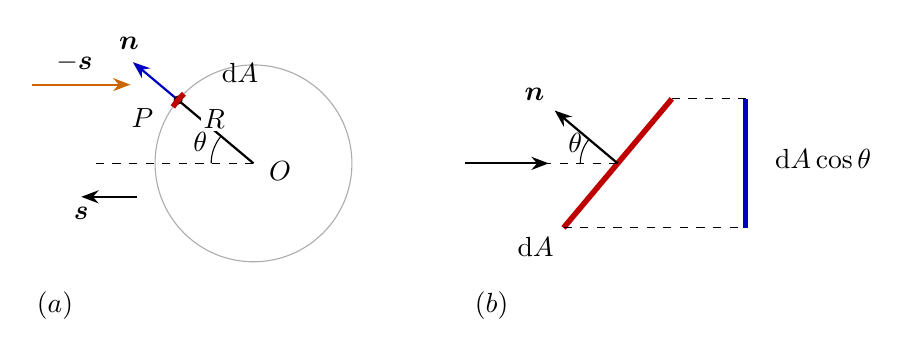
\begin{tikzpicture}[font=\normalsize,scale=1.25]
  \coordinate (O) at (0,0); \coordinate (P) at ({-cos(40)},{sin(40)});
  \draw[gray!65] (O) circle (1);
  \draw[dashed] (O)--(-1.65,0);
  \draw[thick] (O)--(P);
  \draw[arr,blue!75!black] (P)--({-1.6*cos(40)},{1.6*sin(40)});
  \node[anchor=south] at ({-1.65*cos(40)},{1.65*sin(40)}) {$\boldsymbol n$};
  \draw[arr] (-1.18,-.34)--(-1.75,-.34) node[anchor=north] {$\boldsymbol s$};
  \draw[ray] (-2.25,.80)--(-1.25,.80);
  \node[anchor=south] at (-1.82,.83) {$-\boldsymbol s$};
  \draw (O)+(-.43,0) arc[start angle=180,end angle=140,radius=.43];
  \node at (-.54,.22) {$\theta$};
  \node[anchor=west] at (.06,-.08) {$O$};
  \fill (P) circle (1.3pt); \node[anchor=east] at (-.92,.46) {$P$};
  \node[fill=white,inner sep=1pt] at (-.40,.45) {$R$};
  \draw[red!75!black,line width=2pt] ({-cos(35)},{sin(35)}) arc[start angle=145,end angle=135,radius=1];
  \node[anchor=west] at (-.42,.92) {$\mathrm dA$};
  \node[anchor=north west] at (-2.3,-1.20) {$(a)$};
  \begin{scope}[xshift=3.7cm]
    % Length l in the meridian plane; its transverse projection has length l cos(theta).
    \coordinate (A) at (-.55,-.655); \coordinate (B) at (.55,.655);
    \coordinate (Ap) at (1.30,-.655); \coordinate (Bp) at (1.30,.655);
    \draw[red!75!black,line width=2pt] (A)--(B);
    \draw[dashed] (A)--(Ap) (B)--(Bp);
    \draw[blue!75!black,line width=2pt] (Ap)--(Bp);
    \draw[arr] (-1.55,0)--(-.7,0);
    \draw[arr] (0,0)--(-.64,.537) node[anchor=south east] {$\boldsymbol n$};
    \draw[dashed] (0,0)--(-.8,0);
    \draw (0,0)+(-.38,0) arc[start angle=180,end angle=140,radius=.38];
    \node at (-.43,.21) {$\theta$};
    \node[anchor=north east] at (A) {$\mathrm dA$};
    \node[anchor=west] at (1.50,.05) {$\mathrm dA\cos\theta$};
    \node[anchor=north west] at (-1.55,-1.20) {$(b)$};
  \end{scope}
\end{tikzpicture}

% Exact local graph for delta=.001; no visually overlapping .1%-separated states.
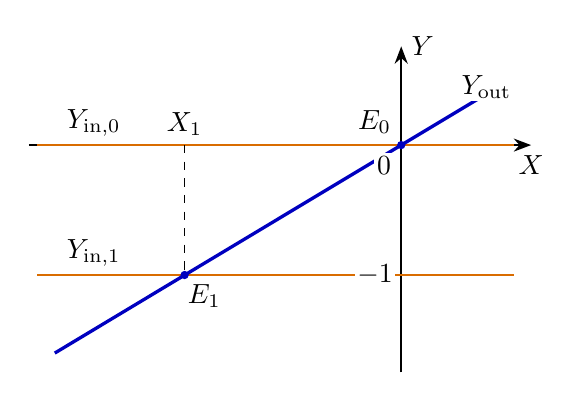
\begin{tikzpicture}[font=\normalsize,x=11cm,y=1.65cm]
  \draw[arr] (-.43,0)--(.15,0) node[anchor=north] {$X$};
  \draw[arr] (0,-1.75)--(0,.76) node[anchor=west] {$Y$};
  \draw[gray!55] (-.42,-1)--(.13,-1);
  \draw[orange!85!black,thick] (-.42,0)--(.13,0);
  \draw[orange!85!black,thick] (-.42,-1)--(.13,-1);
  \draw[blue!75!black,very thick] plot[domain=-.4:.125,samples=61]
    (\x,{4*\x+6*.001*\x^2+4*.001^2*\x^3+.001^3*\x^4});
  \pgfmathsetmacro{\xeq}{-.2500938047}
  \draw[dashed] (\xeq,0)--(\xeq,-1);
  \fill[blue!75!black] (0,0) circle (1.5pt);
  \fill[blue!75!black] (\xeq,-1) circle (1.5pt);
  \node[anchor=south east,fill=white,inner sep=1pt] at (-.008,.06) {$E_0$};
  \node[anchor=north west,fill=white,inner sep=1pt] at (\xeq,-1.05) {$E_1$};
  \node[anchor=south,fill=white,inner sep=1pt] at (\xeq,.05) {$X_1$};
  \node[anchor=north east,fill=white,inner sep=1pt] at (-.008,-.06) {$0$};
  \node[anchor=east,fill=white,inner sep=1pt] at (-.006,-1) {$-1$};
  \node[anchor=south,fill=white,inner sep=1pt] at (-.355,.04) {$Y_{{\rm in},0}$};
  \node[anchor=south,fill=white,inner sep=1pt] at (-.355,-.96) {$Y_{{\rm in},1}$};
  \node[anchor=west,fill=white,inner sep=1pt] at (.066,.45) {$Y_{\rm out}$};
\end{tikzpicture}
\end{document}
